\documentclass{article}
\usepackage[utf8]{inputenc}
\usepackage{array}
\usepackage{multicol}
\usepackage{listings}
\usepackage{amssymb}
\usepackage{enumitem}
\usepackage{graphicx}
\usepackage{amsthm}
\usepackage{hyperref}
\usepackage{tikz}
\usepackage{amssymb}
\usepackage{amsmath}
\usepackage{mathtools}

\usetikzlibrary{automata,positioning}

\begin{document}

\title{Talen \& Automaten \\ Assignment 2}
\date{\today}
\author{Tony Lopar \enspace s1013792 \\TA: Nienke Wessel}
\maketitle

\section*{Exercise 1}
\begin{enumerate}[label=\alph*)]
  \item So we need to find the automate that's the intersection of an automate where $|w|_a$ is not divisible by 3 and an automate where w ends with a.

In order to define M1 where $|w|_a$ is not divisible by 3 we may first create an automate that accepts only words where $|w|_a$ is divisible by 3. After this we could take the complement of this automate to get the automate which only accepts words where $|w|_a$ is not divisible by 3. We can achieve this by changing all the accepting states to non-accepting and the non-accepting to accepting. We see that we can create the following automate that accepts all words where $|w|_a$ is divisible by 3.  \\
\begin{center}
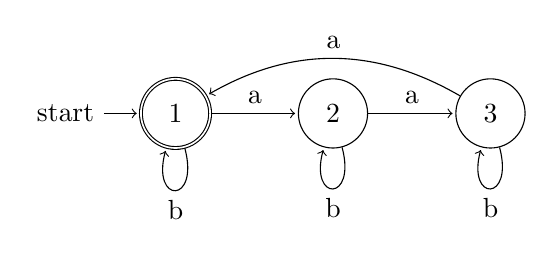
\begin{tikzpicture}[shorten >=1pt,node distance=2cm,on grid,auto]
   \node[state,initial, accepting] (q_1) {$1$};
   \node[state] (q_2) [right=of q_1] {$2$};
   \node[state](q_3) [right=of q_2] {$3$};
    \path[->]
    (q_1) edge  node  {a} (q_2)
          edge [loop below] node {b} ()
    (q_2) edge  node {a} (q_3)
          edge [loop below] node {b} ()
    (q_3) edge [bend right, above] node {a} (q_1)
          edge [loop below] node {b} ();
\end{tikzpicture}
\end{center}

When we take the complement of this automate we find the automate that only accepts words where $|w|_a$ is not divisible by 3. \\
\begin{center}
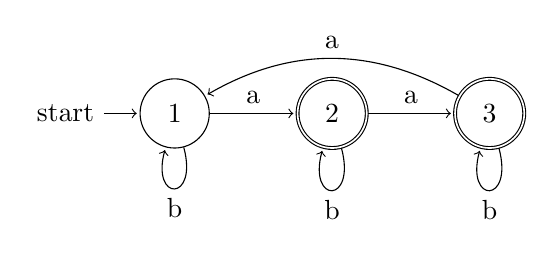
\begin{tikzpicture}[shorten >=1pt,node distance=2cm,on grid,auto]
   \node[state,initial] (q_1) {$1$};
   \node[state, accepting] (q_2) [right=of q_1] {$2$};
   \node[state, accepting](q_3) [right=of q_2] {$3$};
    \path[->]
    (q_1) edge  node  {a} (q_2)
          edge [loop below] node {b} ()
    (q_2) edge  node {a} (q_3)
          edge [loop below] node {b} ()
    (q_3) edge [bend right, above] node {a} (q_1)
          edge [loop below] node {b} ();
\end{tikzpicture}
\end{center}

We will define M2 as an automate where every word ends with an a as: \\
\begin{center}
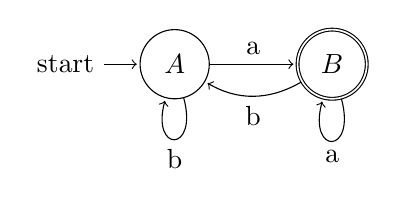
\begin{tikzpicture}[shorten >=1pt,node distance=2cm,on grid,auto]
   \node[state,initial] (q_0)   {$A$};
   \node[state,accepting](q_3) [right=of q_0] {$B$};
    \path[->]
    (q_0) edge  node {a} (q_3)
          edge [loop below] node {b} ()
    (q_3) edge [bend left] node  {b} (q_0)
          edge [loop below] node {a} ();
\end{tikzpicture}
\end{center}

If we take the product of these automata M1 x M2 = M, then this will result in the following automate: \\
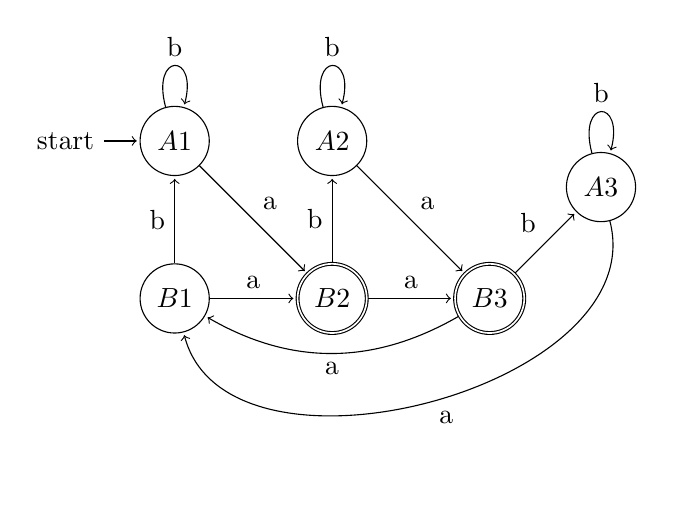
\begin{tikzpicture}[shorten >=1pt,node distance=2cm,on grid,auto]
   \node[state,initial] (A_1)   {$A1$};
   \node[state](A_2) [right=of A_1] {$A2$};

   \node[state](B_1) [below=of A_1] {$B1$};
   \node[state, accepting](B_2) [right=of B_1] {$B2$};
   \node[state, accepting](B_3) [right=of B_2] {$B3$};
   \node[state](A_3) [above right=of B_3] {$A3$};
    \path[->]
    (A_1) edge  node {a} (B_2)
          edge [loop above] node {b} ()
    (A_2) edge  node {a} (B_3)
          edge [loop above] node {b} ()
    (A_3) edge [bend left=90] node {a} (B_1)
          edge [loop above] node {b} ()
    (B_2) edge  node {b} (A_2)
          edge  node {a} (B_3)
    (B_1) edge  node {a} (B_2)
          edge  node {b} (A_1)
    (B_3) edge [bend left] node {a} (B_1)
          edge node {b} (A_3);
\end{tikzpicture}

\item The word abaa is not accepted according to the following accepting computations: \\
\begin{align*}
  \delta^*(A1, abaa) &= \delta^*(\delta (A1, a), baa)       &= \delta^*(B2, baa) \\
                        &= \delta^*(\delta (B2, b), aa)        &= \delta^*(A2, aa) \\
                        &= \delta^*(\delta (A2, a), a)         &= \delta^*(B3, a) \\
                        &= \delta^*(\delta (B3, a), \lambda)   &= \delta^*(B1, \lambda) \\
                        &= B1
\end{align*}
Now we know that abaa ends in $B1$ which is not an accepting state, so the word abaa will not be accepted.

The word ba is accepted according to the following accepting computations: \\
\begin{align*}
\delta^*(A1, ba) &= \delta^*(\delta (A1, b), a)       &= \delta^*(A1, a) \\
                      &= \delta^*(\delta (A1, a), \lambda) &= \delta^*(B2, \lambda) \\
                      &= B2
\end{align*}
Now we know that the automate ends in state $B2$ which is an accepting state. This means the word ba will be accepted.

\item The languages are defined as follows:
\begin{align*}
  L_1 &= \emptyset \\
  % L_1 &= \lambda \\
  L_2 &= \{w | \text{where $|w|_a$ and $|w|_b$ are both an even number} \} \\
  L_3 &= \{w | \text{where $|w|$ is an odd number} \}
\end{align*}
P.S.: \emph{I thought that $L_1$ was the empty set, since $\lambda$ would let the automate remain in the state $q_0$ which is not an accepting state. Because of this I thought that the automate even wouldn't accept $\lambda$ while it has no accepting state.}

\end{enumerate}

\section*{Exercise 2}
\begin{enumerate}[label=\alph*)]
  \item By taking the information given in the exercise we can draw the following automate. \\
  \begin{center}
  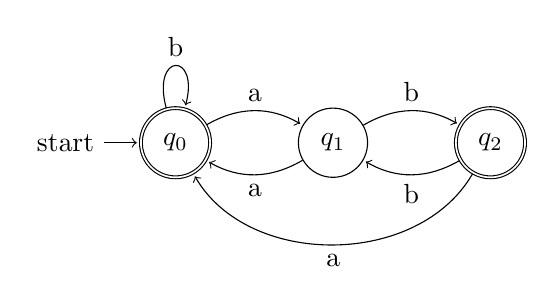
\begin{tikzpicture}[shorten >=1pt,node distance=2cm,on grid,auto]
     \node[state,initial,accepting] (q_0)   {$q_0$};
     \node[state] (q_1) [right=of q_0]  {$q_1$};
     \node[state,accepting](q_2) [right=of q_1] {$q_2$};
      \path[->]
      (q_0) edge [bend left]  node  {a} (q_1)
            edge [loop above] node  {b} ()
      (q_1) edge [bend left]  node  {a} (q_0)
            edge [bend left]  node  {b} (q_2)
      (q_2) edge [bend left=60]  node  {a} (q_0)
            edge [bend left]  node  {b} (q_1);
  \end{tikzpicture}
  \end{center}
  \item In order to construct a regular expression we should try to reduce the number of nodes in the automate. We could first try to remove state $q_1$.
  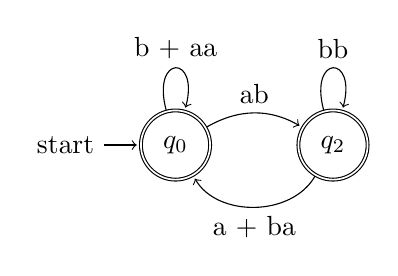
\begin{tikzpicture}[shorten >=1pt,node distance=2cm,on grid,auto]
     \node[state,initial,accepting] (q_0)   {$q_0$};
     \node[state,accepting](q_2) [right=of q_0] {$q_2$};
      \path[->]
      (q_0) edge [bend left]  node  {ab} (q_2)
            edge [loop above] node  {b + aa} ()
      (q_2) edge [bend left=60]  node  {a + ba} (q_0)
            edge [loop above] node  {bb} ();
  \end{tikzpicture}

  Now we have to try to have only one accepting node. We can achieve this by creating an accepting

  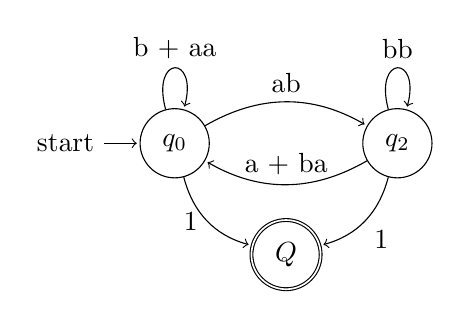
\begin{tikzpicture}[shorten >=1pt,node distance=2cm,on grid,auto]
     \node[state,initial] (q_0)   {$q_0$};
     \node[state,accepting](q) [below right=of q_0] {$Q$};
     \node[state](q_2) [above right=of q] {$q_2$};
      \path[->]
      (q_0) edge [bend left]  node  {ab} (q_2)
            edge [loop above] node  {b + aa} ()
            edge [bend right]  node [left] {1} (q)
      (q_2) edge [bend left]  node [above] {a + ba} (q_0)
            edge [loop above] node  {bb} ()
            edge [bend left]  node  {1} (q);
  \end{tikzpicture}

  We see that this leads to the following expression: \\
\[
  \mathcal{L} (e) = (1 + (b + aa)^* + (ab((bb)^* ba + a))^*)^*(1 + ab(bb)^*)
\]
\end{enumerate}

\end{document}
